\documentclass[12pt,letterpaper]{article}
\usepackage{graphicx,textcomp}
\usepackage{natbib}
\usepackage{setspace}
\usepackage{fullpage}
\usepackage{color}
\usepackage[reqno]{amsmath}
\usepackage{amsthm}
\usepackage{fancyvrb}
\usepackage{amssymb,enumerate}
\usepackage[all]{xy}
\usepackage{endnotes}
\usepackage{lscape}
\newtheorem{com}{Comment}
\usepackage{float}
\usepackage{placeins}
\usepackage{hyperref}
\newtheorem{lem} {Lemma}
\newtheorem{prop}{Proposition}
\newtheorem{thm}{Theorem}
\newtheorem{defn}{Definition}
\newtheorem{cor}{Corollary}
\newtheorem{obs}{Observation}
\usepackage[compact]{titlesec}
\usepackage{dcolumn}
\usepackage{tikz}
\usetikzlibrary{arrows}
\usepackage{multirow}
\usepackage{xcolor}
\newcolumntype{.}{D{.}{.}{-1}}
\newcolumntype{d}[1]{D{.}{.}{#1}}
\definecolor{light-gray}{gray}{0.65}
\usepackage{url}
\usepackage{listings}
\usepackage{color}

\definecolor{codegreen}{rgb}{0,0.6,0}
\definecolor{codegray}{rgb}{0.5,0.5,0.5}
\definecolor{codepurple}{rgb}{0.58,0,0.82}
\definecolor{backcolour}{rgb}{0.95,0.95,0.92}

\lstdefinestyle{mystyle}{
	backgroundcolor=\color{backcolour},
	commentstyle=\color{codegreen},
	keywordstyle=\color{magenta},
	numberstyle=\tiny\color{codegray},
	stringstyle=\color{codepurple},
	basicstyle=\ttfamily\footnotesize,
	breakatwhitespace=false,
	breaklines=true,
	captionpos=b,
	keepspaces=true,
	numbers=left,
	numbersep=5pt,
	showspaces=false,
	showstringspaces=false,
	showtabs=false,
	tabsize=2
}
\lstset{style=mystyle}
\newcommand{\Sref}[1]{Section~\ref{#1}}
\newtheorem{hyp}{Hypothesis}

\title{Problem Set 1}
\date{Due: October 8, 2026\\[0.5em]Emilia Lupi}
\author{Applied Stats/Quant Methods 1}

\begin{document}
	\maketitle
	
	\section*{Instructions}
	\begin{itemize}
		\item Please show your work! You may lose points by simply writing in the answer. If the problem requires you to execute commands in \texttt{R}, please include the code you used to get your answers. Please also include the \texttt{.R} file that contains your code. If you are not sure if work needs to be shown for a particular problem, please ask.
		\item Your homework should be submitted electronically on GitHub.
		\item This problem set is due before 23:59 on Thursday October 8, 2026. No late assignments will be accepted.
	\end{itemize}
	
	\vspace{1cm}
	\section*{Question 1: Education}
	
	A school counselor was curious about the average of IQ of the students in her school and took a random sample of 25 students' IQ scores. The following is the data set:\\
	\vspace{.5cm}
	
	
	\lstinputlisting[language=R, firstline=41, lastline=41]{PS01_solutions_EL.R}
	
	
	
	\vspace{1cm}
	
	\begin{enumerate}
		\item Find a 90\% confidence interval for the average student IQ in the school (As a hint, you first need the mean and SD to create a CI):\\
		
		
		\textbf{Answer.} First, I calculate the descriptive statistics: the sample size, mean, variance, standard deviation, and standard error of the mean.
		
		\lstinputlisting[language=R, firstline=53, lastline=57]{PS01_solutions_EL.R}
		
		The sample size is $n=25$, the mean is $\bar{y}=98.44$, the sample variance is $s^2\approx171.42$, the standard deviation is $s\approx13.09$, and the standard error is $SE\approx2.62$.
		
		Next, I find the critical $t$ score using the \texttt{qt()} function. Since the population standard deviation is unknown, I use the $t$ distribution with $n-1=24$ degrees of freedom. A two-sided 90\% confidence interval leaves 5\% in each tail, so I use the 0.95 quantile.
		
		\lstinputlisting[language=R, firstline=63, lastline=63]{PS01_solutions_EL.R}
		
		The critical value is $t_{0.95,24}\approx1.711$.
		
		The next step is to calculate the lower and upper bounds of the confidence interval by subtracting and adding the critical $t$ score multiplied by the standard error.
		
		\lstinputlisting[language=R, firstline=67, lastline=68]{PS01_solutions_EL.R}
		
		The lower bound is approximately $93.96$ and the upper bound is approximately $102.92$:
		\[
		\bar{y} \pm t_{0.95,24}\frac{s}{\sqrt{n}}
		\approx 98.44 \pm 4.48
		\approx (93.96,\;102.92).
		\]
		
		Finally, I check the step-by-step calculation using the built-in \texttt{t.test()} function, extracting its 90\% confidence interval.
		
		\lstinputlisting[language=R, firstline=73, lastline=73]{PS01_solutions_EL.R}
		
		The built-in function returns the same interval, approximately $(93.96,\;102.92)$, confirming the calculation. We are 90\% confident that this interval contains the population mean IQ of students in the school.
		
		\item Next, the school counselor was curious  whether  the average student IQ in her school is higher than the average IQ score (100) among all the schools in the country.\\
		
		\noindent Using the same sample, conduct the appropriate hypothesis test with $\alpha=0.05$.\\
		
		
		\textbf{Answer.} I conduct a one-sided, upper-tail $t$ test.
		
		\medskip
		\noindent\textbf{Step 1: Assumptions.}
		IQ is quantitative, and the 25 students were randomly sampled. Observations are assumed independent. With this small sample, I assume that population IQ is approximately normally distributed, without strong skewness or extreme outliers. The population standard deviation is unknown, so I use a $t$ test with $n-1=24$ degrees of freedom.
		
		\medskip
		\noindent\textbf{Step 2: State the hypotheses.}
		Let $\mu$ denote the population mean of the IQ of students in the school. The hypotheses are:
		\[
		H_0:\mu\leq100,\qquad H_A:\mu>100.
		\]
		The significance level is $\alpha=0.05$.
		
		\medskip
		\noindent\textbf{Step 3: Calculate the test statistic.}
		I subtract the hypothesized mean from the sample mean and divide by the estimated standard error:
		\[
		t=\frac{\bar{y}-100}{s/\sqrt{n}}.
		\]
		\lstinputlisting[language=R, firstline=98, lastline=99]{PS01_solutions_EL.R}
		The resulting test statistic is approximately $-0.60$.
		
		\medskip
		\noindent\textbf{Step 4: Calculate the p-value.}
		Assuming the population mean IQ is 100, the $p$-value is the probability of obtaining a $t$ statistic equal to or greater than the one observed. Since the alternative hypothesis is $\mu>100$, I calculate this probability in the upper tail of the $t$ distribution with 24 degrees of freedom.
		\lstinputlisting[language=R, firstline=102, lastline=103]{PS01_solutions_EL.R}
		The $p$-value is approximately $0.72$.
		
		\medskip
		\noindent\textbf{Step 5: Draw a conclusion.}
		Since $p\approx0.72>0.05$, I fail to reject $H_0$. There is insufficient evidence that the population mean IQ of students in the school is higher than 100.
		
		\medskip
		\noindent Finally, I check the calculations using the built-in \texttt{t.test()} function:
		\lstinputlisting[language=R, firstline=110, lastline=110]{PS01_solutions_EL.R}
		
		The built-in function gives the same test statistic and p-value as the step-by-step hypothesis test, confirming the same conclusion.
		
	\end{enumerate}
	
	\newpage
	
	\section*{Question 2: Political Economy}
	
	\noindent Researchers are curious about what affects the amount of money communities spend on addressing homelessness. The following variables constitute our data set about social welfare expenditures in the USA. \\
	\vspace{.5cm}
	
	
	\begin{tabular}{r|l}
		\texttt{State} &\emph{50 states in US} \\
		\texttt{Y} & \emph{per capita expenditure on shelters/housing assistance in state}\\
		\texttt{X1} &\emph{per capita personal income in state} \\
		\texttt{X2} &  \emph{Number of residents per 100,000 that are "financially insecure" in state}\\
		\texttt{X3} &  \emph{Number of people per thousand residing in urban areas in state} \\
		\texttt{Region} &  \emph{1=Northeast, 2= North Central, 3= South, 4=West} \\
	\end{tabular}
	
	\vspace{.5cm}
	\noindent Explore the \texttt{expenditure} data set and import data into \texttt{R}.
	\vspace{.5cm}
	
	Region is a category rather than a numerical quantity, so I convert it into a labelled factor.
	
	\lstinputlisting[language=R, firstline=132, lastline=134]{PS01_solutions_EL.R}
	
	\vspace{.5cm}
	\begin{itemize}
		
		\item
		Please plot the relationships among \emph{Y}, \emph{X1}, \emph{X2}, and \emph{X3}? What are the correlations among them (you just need to describe the graph and the relationships among them)?\\
		
		\textbf{Answer.} I use scatter plots because all four variables are numerical. I use \texttt{par()} to arrange the six plots in a $2\times3$ grid and nested \texttt{for} loops to plot each pair to avoid repeating the plotting code. I also use \texttt{abline()} with \texttt{lm()} to add a least-squares regression line to each plot, making the overall linear trend easier to see.
		
		\lstinputlisting[language=R, firstline=144, lastline=184]{PS01_solutions_EL.R}
		
		\begin{figure}[H]
			\centering
			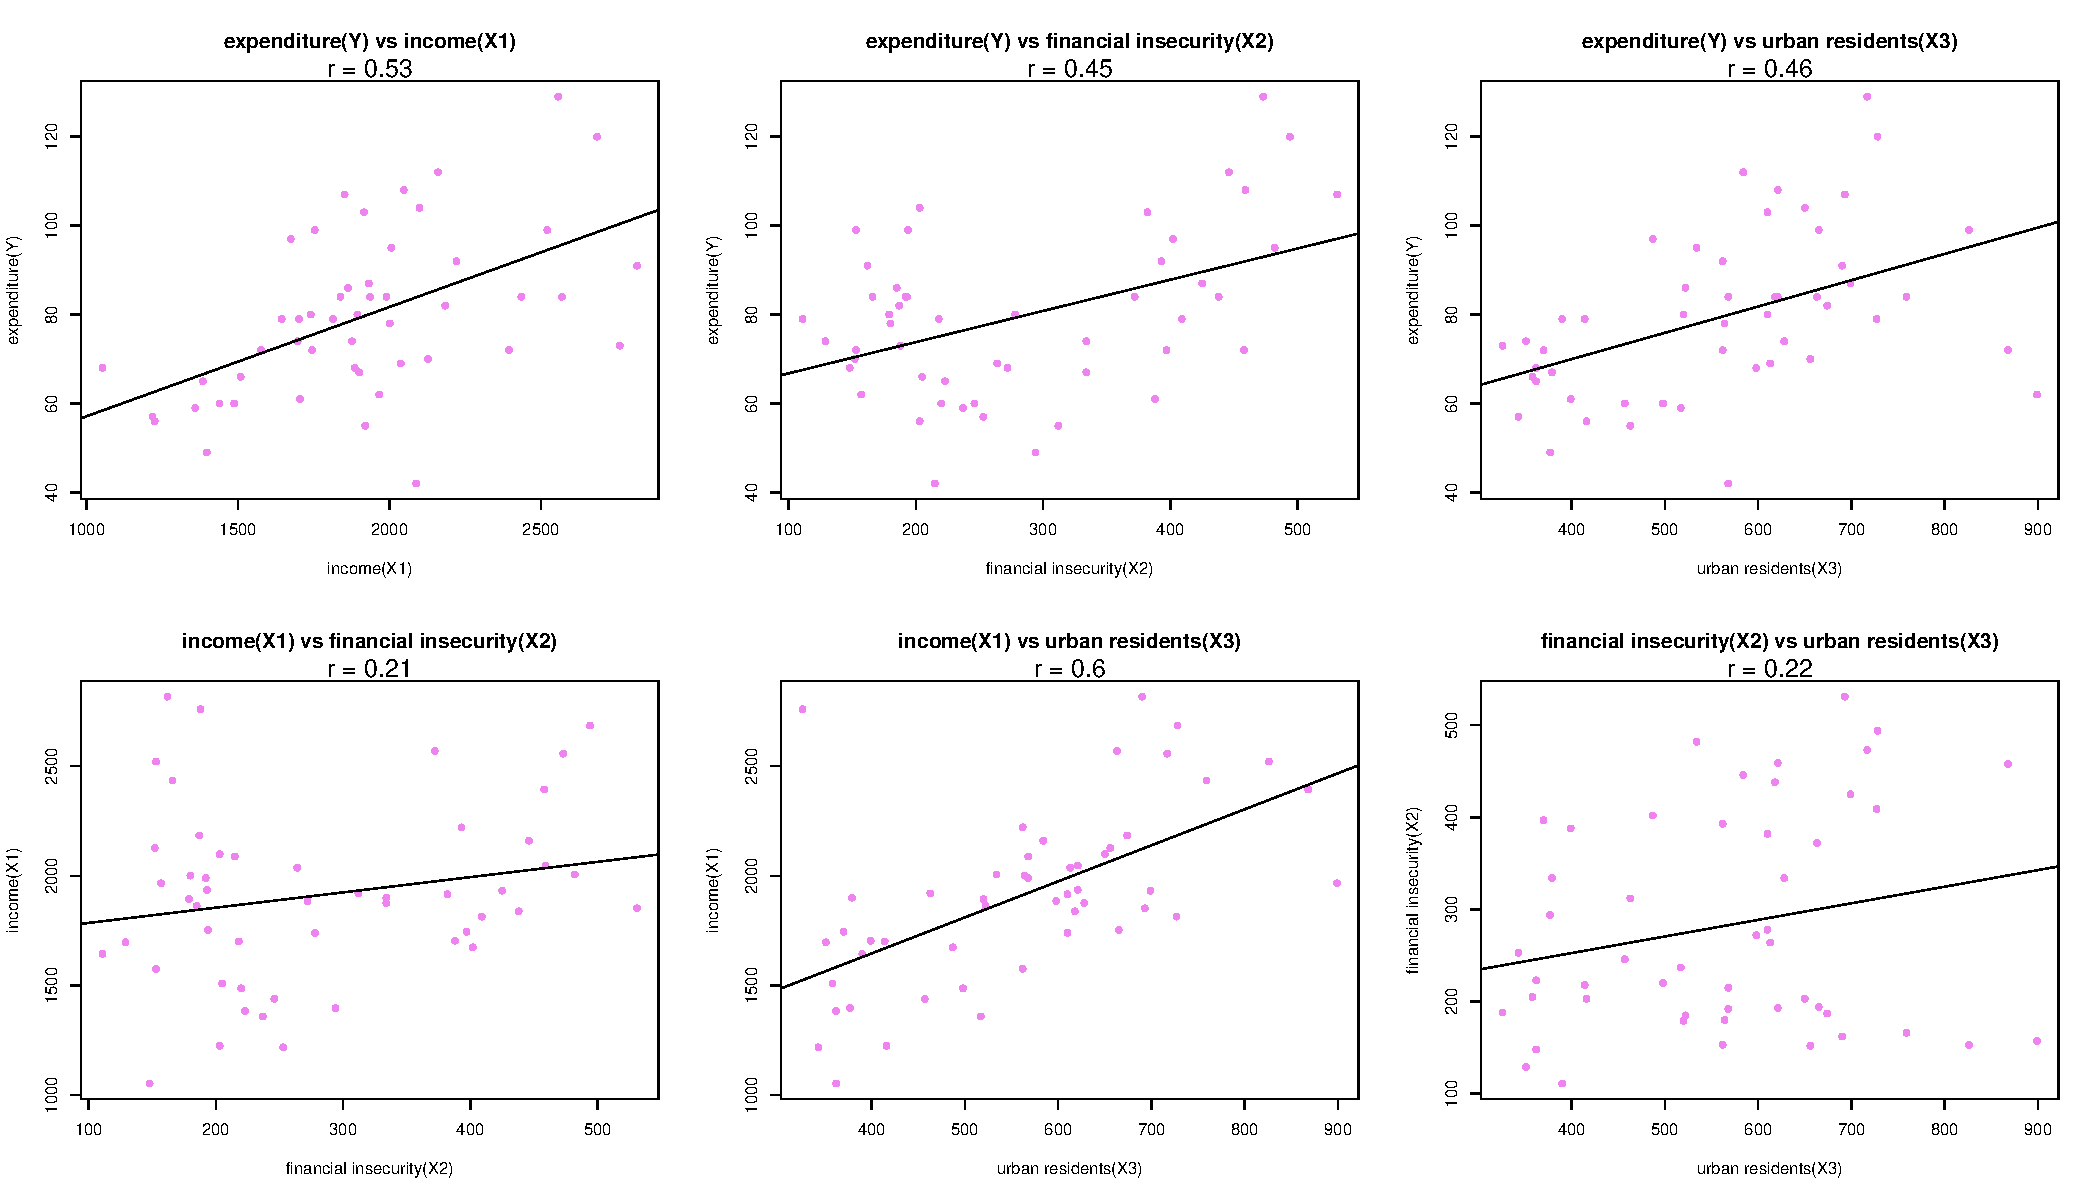
\includegraphics[width=0.95\linewidth]{P1_relationships_expenditure.pdf}
			\caption{Pairwise relationships among expenditure, income, financial insecurity, and urban population.}
		\end{figure}
		
		The pairwise correlations are positive. Expenditure ($Y$) has moderate positive associations with income ($X1$, $r=0.53$), financial insecurity ($X2$, $r=0.45$), and urban population ($X3$, $r=0.46$). This suggests that states with higher per capita income, higher rates of financial insecurity, or larger proportions of urban residents tend to spend more per capita on housing assistance.
		
		Among the explanatory variables, income and urban population have the strongest correlation ($r=0.60$), indicating that more urbanised states tend to have higher per capita incomes. Financial insecurity is weakly correlated with income ($r=0.21$) and urban population ($r=0.22$), so these relationships show only slight upward trends, with substantial variation.
		
		\vspace{.5cm}
		\item
		Please plot the relationship between \emph{Y} and \emph{Region}? On average, which region has the highest per capita expenditure on housing assistance?\\
		
		\textbf{Answer.} I use a boxplot to compare the distribution of expenditure, a numerical variable, across regions, a categorical variable. The line inside each box represents the median, while the box contains the middle 50\% of observations. Differences in box and whisker lengths indicate differences in the spread of expenditure.
		
		\lstinputlisting[language=R, firstline=199, lastline=205]{PS01_solutions_EL.R}
		
		\begin{figure}[H]
			\centering
			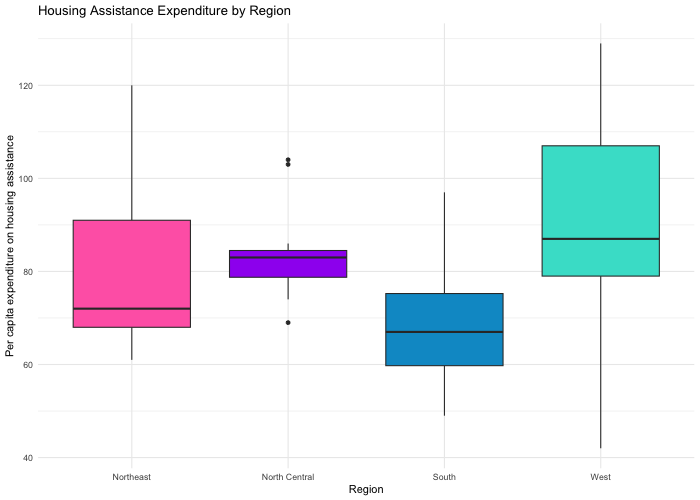
\includegraphics[width=0.95\linewidth]{P2Q2_boxplot_Y_Region.png}
			\caption{Distribution of per capita housing assistance expenditure by region.}
		\end{figure}
		
		
		From Figure 2, we can see that the West has the highest median per capita expenditure in housing assistance, followed by North Central, Northeast and lastly South. Additionally, the West also has the widest interquartile range, which indicates great variation across states. On the other hand, the North Central region has the smallest interquartile range, so its middle 50\% of observations are concentrated around the median. However, it has three potential outliers: one low value near 69 and two high values around 103–104. The Northeast and South show intermediate variability, with the Northeast having a wider interquartile range than the South.
		
		To compare the means specifically, rather than the medians shown in the boxplot, I calculate average expenditure for each region and store the results in \texttt{region\_means}.
		
		\lstinputlisting[language=R, firstline=209, lastline=209]{PS01_solutions_EL.R}
		
		
% Table created by stargazer v.5.2.3 by Marek Hlavac, Social Policy Institute. E-mail: marek.hlavac at gmail.com
% Date and time: Wed, Oct 07, 2026 - 14:28:36
\begin{table}[!htbp] \centering 
  \caption{Average Housing Assistance Expenditure by Region} 
  \label{tab:region_means} 
\begin{tabular}{@{\extracolsep{5pt}} cc} 
\\[-1.8ex]\hline 
\hline \\[-1.8ex] 
Region & Y \\ 
\hline \\[-1.8ex] 
Northeast & $79.4$ \\ 
North Central & $83.9$ \\ 
South & $69.2$ \\ 
West & $88.3$ \\ 
\hline \\[-1.8ex] 
\end{tabular} 
\end{table} 

		\FloatBarrier
		
		On average, the West spends the most per capita on housing assistance (88.3), followed by North Central (83.9), the Northeast (79.4), and the South (69.2).
		
		I use the \texttt{stargazer} package to export the regional means as a LaTeX table and include it in this document.
		
		\vspace{.5cm}
		\item
		Please plot the relationship between \emph{Y} and \emph{X1}? Describe this graph and the relationship. Reproduce the above graph including one more variable \emph{Region} and display different regions with different types of symbols and colors.\\
		
		\textbf{Answer.} A scatter plot is appropriate for examining the relationship between income ($X1$) and expenditure ($Y$), since both variables are numerical. I use the \texttt{ggplot2} package to create the plot and add a fitted regression line to show the overall linear trend.
		
		\lstinputlisting[language=R, firstline=231, lastline=231]{PS01_solutions_EL.R}
		
		\lstinputlisting[language=R, firstline=234, lastline=245]{PS01_solutions_EL.R}
		
		\begin{figure}[H]
			\centering
			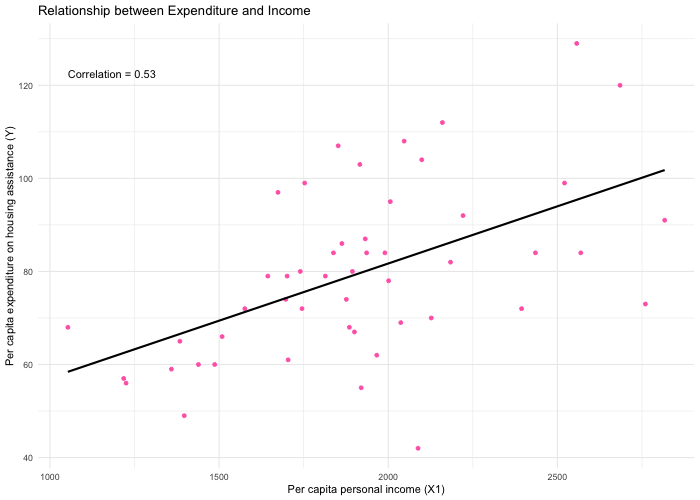
\includegraphics[width=0.95\linewidth]{P2Q3_Y_X1.png}
			\caption{Relationship between per capita income and housing assistance expenditure.}
		\end{figure}
		
		Income and expenditure have a moderate positive relationship ($r\approx0.53$). States with higher per capita income tend to spend more per capita on housing assistance, although there is substantial variation around the fitted line.\\
		
		\textbf{Adding Region.} I distinguish regions using both colors and symbols.
		
		\lstinputlisting[language=R, firstline=253, lastline=260]{PS01_solutions_EL.R}
		
		\begin{figure}[H]
			\centering
			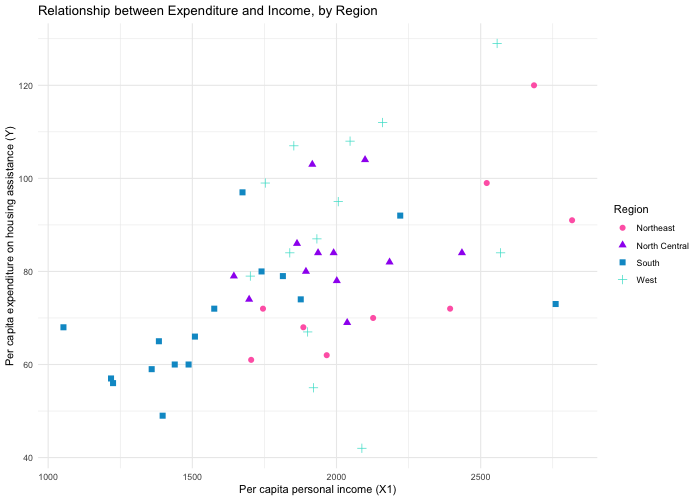
\includegraphics[width=0.95\linewidth]{P2Q3_Y_X1_by_Region.png}
			\caption{Income and expenditure, with regions identified by color and symbol.}
		\end{figure}
		
		The regional groups are partly clustered: Southern states tend to have lower income and expenditure, while Northeastern states tend to have higher incomes. North Central and West regions mostly fall in the middle part of graph. Figure 4 suggests that regional differences may contribute to the overall association.
		
	\end{itemize}
	
	
\end{document}
